\tikzstyle{vertex}=[circle,fill=black!25,minimum size=10pt,inner sep=2pt]
\tikzstyle{Nvertex}=[circle,fill=white!25,minimum size=10pt,inner sep=2pt]
\tikzstyle{LabelStyle}=[fill=white,sloped]

\tikzstyle{big_vertex}=[circle,fill=red!15,minimum size=50pt,inner sep=2pt,draw=black!50]
\tikzstyle{med_vertex}=[circle,fill=red!10,minimum size=35pt,inner sep=2pt,draw=black!50]

\tikzstyle{macrostate_vertex}=[inner sep=3pt,draw=black!70]


\newcommand{\vertexshiftamount}{2.5}
\newcommand{\tikzpicscale}{1.5}

\newcommand{\TIKZenergylevel}{

  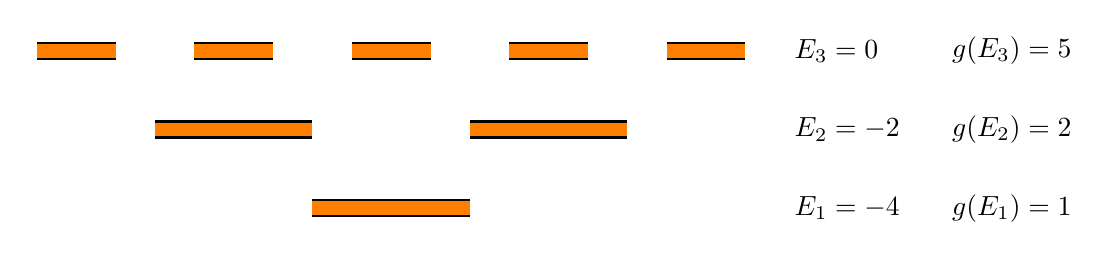
\begin{tikzpicture}
    \tikzset{level/.style   = {thick,
        double          = orange,
        double distance = 5pt}}
    
    \def\Espace{9};
    \def\Gspace{11};
    
    % Draw the energy levels.
    \draw[level] (3,0)  -- (5,0) node[right]{};
    \draw[] (\Espace,0) node[right] {$E_1=-4$};
    \draw[] (\Gspace,0) node[right] {$g(E_1)=1$};
    
    \draw[level] (1,1) -- (3,1) node[right] {};
    \draw[level] (5,1) -- (7,1) node[right] {};
    \draw[] (\Espace,1) node[right] {$E_2=-2$};
    \draw[] (\Gspace,1) node[right] {$g(E_2)=2$};
    
    \def\v{.5}; 
    \draw[level] (-1+\v,2) -- (0+\v,2) node[right] {};
    \draw[level] (1+\v,2) -- (2+\v,2) node[right] {};
    \draw[level] (3+\v,2) -- (4+\v,2) node[right] {};
    \draw[level] (5+\v,2) -- (6+\v,2) node[right] {};
    \draw[level] (7+\v,2) -- (8+\v,2) node[right] {};
    \draw[] (\Espace,2) node[right] {$E_3=0$};
    \draw[] (\Gspace,2) node[right] {$g(E_3)=5$};
  \end{tikzpicture}
}

\newcommand{\TIKZenergylevelSHORT}{

  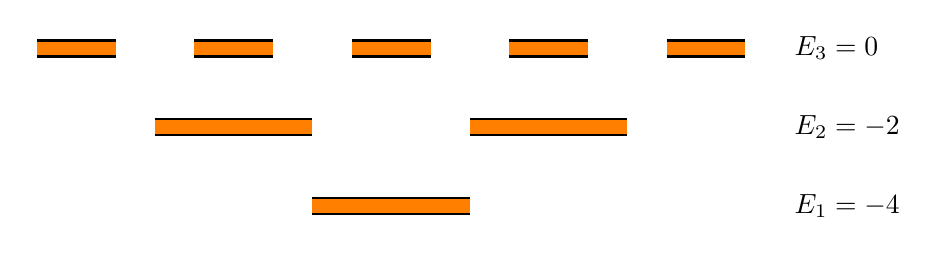
\begin{tikzpicture}
    \tikzset{level/.style   = {thick,
        double          = orange,
        double distance = 5pt,
        scale = 1.
        }}
    
    \def\Espace{9};
    \def\Gspace{11};
    
    % Draw the energy levels.
    \draw[level] (3,0)  -- (5,0) node[right]{};
    \draw[] (\Espace,0) node[right] {$E_1=-4$};
   
    \draw[level] (1,1) -- (3,1) node[right] {};
    \draw[level] (5,1) -- (7,1) node[right] {};
    \draw[] (\Espace,1) node[right] {$E_2=-2$};
    
    \def\v{.5}; 
    \draw[level] (-1+\v,2) -- (0+\v,2) node[right] {};
    \draw[level] (1+\v,2) -- (2+\v,2) node[right] {};
    \draw[level] (3+\v,2) -- (4+\v,2) node[right] {};
    \draw[level] (5+\v,2) -- (6+\v,2) node[right] {};
    \draw[level] (7+\v,2) -- (8+\v,2) node[right] {};
    \draw[] (\Espace,2) node[right] {$E_3=0$};
  \end{tikzpicture}
}


\newcommand{\TIKZgraphABC}{
  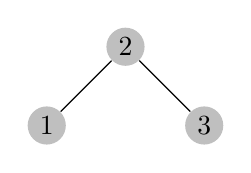
\begin{tikzpicture}[shorten >=1pt,->]
    \tikzstyle{vertex}=[circle,fill=black!25,minimum size=12pt,inner sep=2pt]
    \node[vertex] (G_1) at (-1,-1) {1};
    \node[vertex] (G_2) at (0,0)   {2};
    \node[vertex] (G_3) at (1,-1)  {3};
    \draw (G_1) -- (G_2) -- (G_3) -- cycle;
  \end{tikzpicture}
}

\newcommand{\TIKZgraphAB}{
  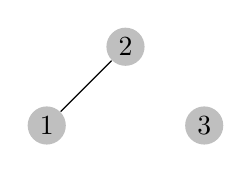
\begin{tikzpicture}[shorten >=1pt,->]
    \tikzstyle{vertex}=[circle,fill=black!25,minimum size=12pt,inner sep=2pt]
    \node[vertex] (G_1) at (-1,-1) {1};
    \node[vertex] (G_2) at (0,0)   {2};
    \node[vertex] (G_3) at (1,-1)  {3};
    \draw (G_1) -- (G_2) -- cycle;
  \end{tikzpicture}
}

\newcommand{\TIKZgraphBC}{
  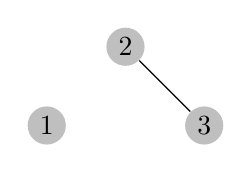
\begin{tikzpicture}[shorten >=1pt,->]
    \tikzstyle{vertex}=[circle,fill=black!25,minimum size=12pt,inner sep=2pt]
    \node[vertex] (G_1) at (-1,-1) {1};
    \node[vertex] (G_2) at (0,0)   {2};
    \node[vertex] (G_3) at (1,-1)  {3};
    \draw (G_2) -- (G_3) -- cycle;
  \end{tikzpicture}
}

\newcommand{\TIKZgraphC}{
  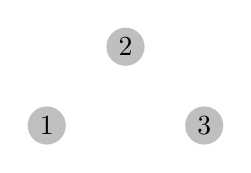
\begin{tikzpicture}[shorten >=1pt,->]
    \tikzstyle{vertex}=[circle,fill=black!25,minimum size=12pt,inner sep=2pt]
    \node[vertex] (G_1) at (-1,-1) {1};
    \node[vertex] (G_2) at (0,0)   {2};
    \node[vertex] (G_3) at (1,-1)  {3};
  \end{tikzpicture}
}


\newcommand{\TIKZgraphoneline}{
  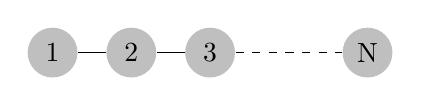
\begin{tikzpicture}[shorten >=1pt,->]
    \tikzstyle{vertex}=[circle,fill=black!25,minimum size=18pt,inner sep=2pt]
    \node[vertex] (G1) at (0,0)   {1};
    \node[vertex] (G2) at (1,0)   {2};
    \node[vertex] (G3) at (2,0)   {3};
    \node[vertex] (GN) at (4,0)   {N};
    \draw (G1) -- (G2) -- (G3) -- cycle;
    \draw[dashed] (G3) -- (GN) -- cycle;
  \end{tikzpicture}
}


\newcommand{\TIKZgraphtwoline}{
  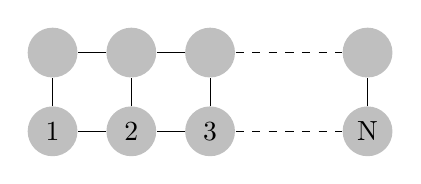
\begin{tikzpicture}[shorten >=1pt,->]
    \tikzstyle{vertex}=[circle,fill=black!25,minimum size=18pt,inner sep=2pt]
    \node[vertex] (G1) at (0,0)   {1};
    \node[vertex] (G2) at (1,0)   {2};
    \node[vertex] (G3) at (2,0)   {3};
    \node[vertex] (GN) at (4,0)   {N};
    \draw (G1) -- (G2) -- (G3) -- cycle;
    \draw[dashed] (G3) -- (GN) -- cycle;

    \node[vertex] (GN1) at (0,1)   {};
    \node[vertex] (GN2) at (1,1)   {};
    \node[vertex] (GN3) at (2,1)   {};
    \node[vertex] (G2N) at (4,1)   {};
    
    \draw (GN1) -- (GN2) -- (GN3) -- cycle;
    \draw (GN) -- (G2N) -- cycle;
    \draw (G1) -- (GN1) -- cycle;
    \draw (G2) -- (GN2) -- cycle;
    \draw (G3) -- (GN3) -- cycle;
    \draw (GN) -- (G2N) -- cycle;

    \draw[dashed] (GN3) -- (G2N) -- cycle;


  \end{tikzpicture}
}



\newcommand{\TIKZtwoladdera}{
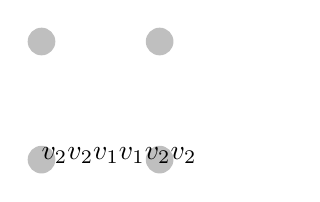
\begin{tikzpicture}[scale=\tikzpicscale]
    \node[vertex] (G1) at (0,0)   {};
    \node[vertex] (G2) at (1,0)   {};
    \node[vertex] (GA) at (0,1)   {};
    \node[vertex] (GB) at (1,1)   {};
	 \Edge[label=$v_2$](G1)(G2)
	 \Edge[label=$v_2$](GA)(GB)
	 \Edge[label=$v_1$](G1)(GA)
	 \Edge[label=$v_1$](G2)(GB)
    \node[Nvertex] (G3) at (2,0)   {};
    \node[Nvertex] (GC) at (2,1)   {};
	 \tikzstyle{EdgeStyle}=[dashed]
	 \Edge[label=$v_2$](G2)(G3)
	 \Edge[label=$v_2$](GB)(GC)
\end{tikzpicture}
}

\newcommand{\TIKZtwoladderb}{
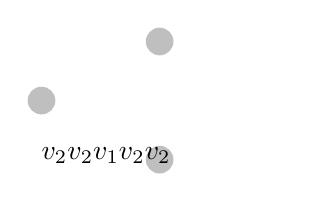
\begin{tikzpicture}[scale=\tikzpicscale]
    \node[vertex] (G2) at (1,0)   {};
    \node[vertex] (GB) at (1,1)   {};
    \node[vertex] (G1A) at (0,.5)   {};
	 \Edge[label=$v_2$](G1A)(G2)
	 \Edge[label=$v_2$](G1A)(GB)
	 \Edge[label=$v_1$](G2)(GB)
    \node[Nvertex] (G3) at (2,0)   {};
    \node[Nvertex] (GC) at (2,1)   {};
	 \tikzstyle{EdgeStyle}=[dashed]
	 \Edge[label=$v_2$](G2)(G3)
	 \Edge[label=$v_2$](GB)(GC)
\end{tikzpicture}
}

\newcommand{\TIKZtwoladderc}{
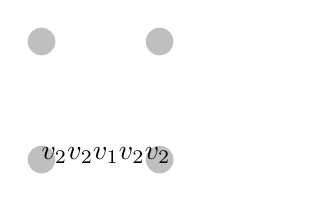
\begin{tikzpicture}[scale=\tikzpicscale]
    \node[vertex] (G1) at (0,0)   {};
    \node[vertex] (G2) at (1,0)   {};
    \node[vertex] (GA) at (0,1)   {};
    \node[vertex] (GB) at (1,1)   {};
	 \Edge[label=$v_2$](G1)(G2)
	 \Edge[label=$v_2$](GA)(GB)
	 %\Edge[label=$v_1$](G1)(GA)
	 \Edge[label=$v_1$](G2)(GB)
    \node[Nvertex] (G3) at (2,0)   {};
    \node[Nvertex] (GC) at (2,1)   {};
	 \tikzstyle{EdgeStyle}=[dashed]
	 \Edge[label=$v_2$](G2)(G3)
	 \Edge[label=$v_2$](GB)(GC)
\end{tikzpicture}
}

\newcommand{\TIKZtwoladderd}{
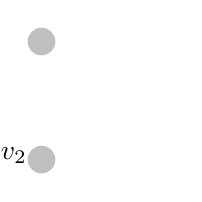
\begin{tikzpicture}[scale=\tikzpicscale]
    \node[vertex] (G2) at (1,0)   {};
    \node[vertex] (GB) at (1,1)   {};
	 %\Edge[label=$v_1$](G1)(GA)
	\tikzstyle{EdgeStyle}=[bend left]
	\Edge[label=$v_2$](G2)(GB)
  	\tikzstyle{EdgeStyle}=[bend right]
	\Edge[label=$v_1$](G2)(GB)
    \node[Nvertex] (G3) at (2,0)   {};
    \node[Nvertex] (GC) at (2,1)   {};
	 \tikzstyle{EdgeStyle}=[dashed]
	 \Edge[label=$v_2$](G2)(G3)
	 \Edge[label=$v_2$](GB)(GC)
\end{tikzpicture}
}

\newcommand{\TIKZtwoladdere}{
\begin{tikzpicture}[scale=\tikzpicscale]
    \node[vertex] (G2B) at (1,.5)   {};
	 %\Edge[label=$v_1$](G1)(GA)
	\tikzstyle{EdgeStyle}=[loop above]
	\Edge[label=$v_1$](G2B)(G2B)
   \node[Nvertex] (G3) at (2,0)   {};
   \node[Nvertex] (GC) at (2,1)   {};
	\tikzstyle{EdgeStyle}=[dashed]
	\Edge[label=$v_2$](G2B)(G3)
	\Edge[label=$v_2$](G2B)(GC)
\end{tikzpicture}
}

\newcommand{\TIKZtwoladderf}{
\begin{tikzpicture}[scale=\tikzpicscale]
    \node[vertex] (G2B) at (1,.5)   {};
   \node[Nvertex] (G3) at (2,0)   {};
   \node[Nvertex] (GC) at (2,1)   {};
	\tikzstyle{EdgeStyle}=[dashed]
	\Edge[label=$v_2$](G2B)(G3)
	\Edge[label=$v_2$](G2B)(GC)
\end{tikzpicture}
}

\newcommand{\TIKZthreeladderA}{
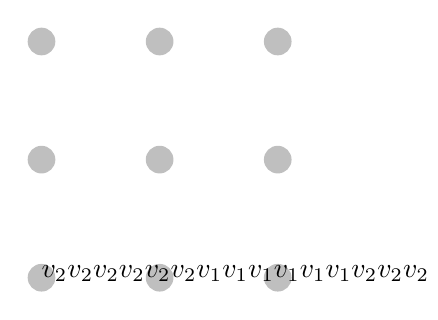
\begin{tikzpicture}[scale=\tikzpicscale]
    \node[vertex] (00) at (0,0)   {};
    \node[vertex] (10) at (1,0)   {};
	 \node[vertex] (20) at (2,0)   {};
    \node[vertex] (01) at (0,1)   {};
    \node[vertex] (11) at (1,1)   {};
    \node[vertex] (21) at (2,1)   {};
    \node[vertex] (02) at (0,2)   {};
    \node[vertex] (12) at (1,2)   {};
    \node[vertex] (22) at (2,2)   {};
	 \Edge[label=$v_2$](00)(10)
	 \Edge[label=$v_2$](10)(20)
	 \Edge[label=$v_2$](01)(11)
	 \Edge[label=$v_2$](11)(21)
	 \Edge[label=$v_2$](02)(12)
	 \Edge[label=$v_2$](12)(22)	
	 \Edge[label=$v_1$](00)(01)
	 \Edge[label=$v_1$](10)(11)
	 \Edge[label=$v_1$](20)(21)
 	 \Edge[label=$v_1$](21)(22)
 	 \Edge[label=$v_1$](11)(12)
 	 \Edge[label=$v_1$](01)(02)
    \node[Nvertex] (n30) at (3,0)   {};
    \node[Nvertex] (n31) at (3,1)   {};
    \node[Nvertex] (n32) at (3,2)   {};
	 \tikzstyle{EdgeStyle}=[dashed]
	 \Edge[label=$v_2$](20)(n30)
	 \Edge[label=$v_2$](21)(n31)
 	 \Edge[label=$v_2$](22)(n32)
\end{tikzpicture}
}

\newcommand{\TIKZthreeladderB}{
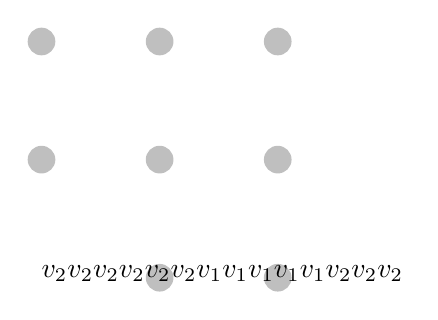
\begin{tikzpicture}[scale=\tikzpicscale]
%    \node[vertex] (00) at (0,0)   {};
    \node[vertex] (10) at (1,0)   {};
	 \node[vertex] (20) at (2,0)   {};
    \node[vertex] (01) at (0,1)   {};
    \node[vertex] (11) at (1,1)   {};
    \node[vertex] (21) at (2,1)   {};
    \node[vertex] (02) at (0,2)   {};
    \node[vertex] (12) at (1,2)   {};
    \node[vertex] (22) at (2,2)   {};
	 \Edge[label=$v_2$](01)(10)
	 \Edge[label=$v_2$](10)(20)
	 \Edge[label=$v_2$](01)(11)
	 \Edge[label=$v_2$](11)(21)
	 \Edge[label=$v_2$](02)(12)
	 \Edge[label=$v_2$](12)(22)	
%)	 \Edge[label=$v_1$](00)(01)
	 \Edge[label=$v_1$](10)(11)
	 \Edge[label=$v_1$](20)(21)
 	 \Edge[label=$v_1$](21)(22)
 	 \Edge[label=$v_1$](11)(12)
 	 \Edge[label=$v_1$](01)(02)
    \node[Nvertex] (n30) at (3,0)   {};
    \node[Nvertex] (n31) at (3,1)   {};
    \node[Nvertex] (n32) at (3,2)   {};
	 \tikzstyle{EdgeStyle}=[dashed]
	 \Edge[label=$v_2$](20)(n30)
	 \Edge[label=$v_2$](21)(n31)
 	 \Edge[label=$v_2$](22)(n32)
\end{tikzpicture}
}

\newcommand{\TIKZthreeladderC}{
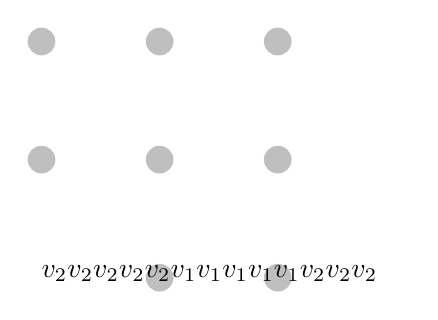
\begin{tikzpicture}[scale=\tikzpicscale]
%    \node[vertex] (00) at (0,0)   {};
    \node[vertex] (10) at (1,0)   {};
	 \node[vertex] (20) at (2,0)   {};
    \node[vertex] (01) at (0,1)   {};
    \node[vertex] (11) at (1,1)   {};
    \node[vertex] (21) at (2,1)   {};
    \node[vertex] (02) at (0,2)   {};
    \node[vertex] (12) at (1,2)   {};
    \node[vertex] (22) at (2,2)   {};
%	 \Edge[label=$v_2$](01)(10)
	 \Edge[label=$v_2$](10)(20)
	 \Edge[label=$v_2$](01)(11)
	 \Edge[label=$v_2$](11)(21)
	 \Edge[label=$v_2$](02)(12)
	 \Edge[label=$v_2$](12)(22)	
%)	 \Edge[label=$v_1$](00)(01)
	 \Edge[label=$v_1$](10)(11)
	 \Edge[label=$v_1$](20)(21)
 	 \Edge[label=$v_1$](21)(22)
 	 \Edge[label=$v_1$](11)(12)
 	 \Edge[label=$v_1$](01)(02)
    \node[Nvertex] (n30) at (3,0)   {};
    \node[Nvertex] (n31) at (3,1)   {};
    \node[Nvertex] (n32) at (3,2)   {};
	 \tikzstyle{EdgeStyle}=[dashed]
	 \Edge[label=$v_2$](20)(n30)
	 \Edge[label=$v_2$](21)(n31)
 	 \Edge[label=$v_2$](22)(n32)
\end{tikzpicture}
}

\newcommand{\TIKZthreeladderD}{
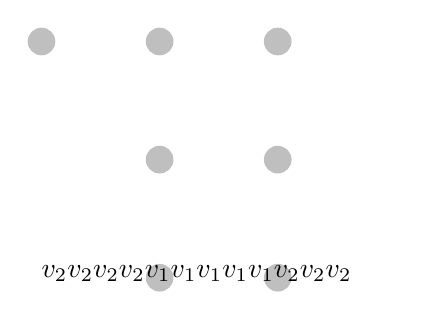
\begin{tikzpicture}[scale=\tikzpicscale]
%    \node[vertex] (00) at (0,0)   {};
    \node[vertex] (10) at (1,0)   {};
	 \node[vertex] (20) at (2,0)   {};
%    \node[vertex] (01) at (0,1)   {};
    \node[vertex] (11) at (1,1)   {};
    \node[vertex] (21) at (2,1)   {};
    \node[vertex] (02) at (0,2)   {};
    \node[vertex] (12) at (1,2)   {};
    \node[vertex] (22) at (2,2)   {};
%	 \Edge[label=$v_2$](01)(10)
	 \Edge[label=$v_2$](10)(20)
%	 \Edge[label=$v_2$](01)(11)
	 \Edge[label=$v_2$](11)(21)
	 \Edge[label=$v_2$](02)(12)
	 \Edge[label=$v_2$](12)(22)	
%)	 \Edge[label=$v_1$](00)(01)
	 \Edge[label=$v_1$](10)(11)
	 \Edge[label=$v_1$](20)(21)
 	 \Edge[label=$v_1$](21)(22)
 	 \Edge[label=$v_1$](11)(12)
 	 \Edge[label=$v_1$](11)(02)
    \node[Nvertex] (n30) at (3,0)   {};
    \node[Nvertex] (n31) at (3,1)   {};
    \node[Nvertex] (n32) at (3,2)   {};
	 \tikzstyle{EdgeStyle}=[dashed]
	 \Edge[label=$v_2$](20)(n30)
	 \Edge[label=$v_2$](21)(n31)
 	 \Edge[label=$v_2$](22)(n32)
\end{tikzpicture}
}

\newcommand{\TIKZthreeladderE}{
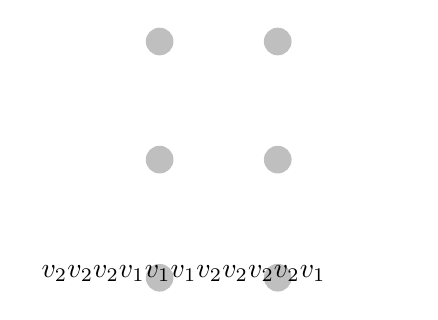
\begin{tikzpicture}[scale=\tikzpicscale]
    \node[Nvertex] (00) at (0,0)   {};
    \node[vertex] (10) at (1,0)   {};
	 \node[vertex] (20) at (2,0)   {};
%    \node[vertex] (01) at (0,1)   {};
    \node[vertex] (11) at (1,1)   {};
    \node[vertex] (21) at (2,1)   {};
%    \node[vertex] (02) at (0,2)   {};
    \node[vertex] (12) at (1,2)   {};
    \node[vertex] (22) at (2,2)   {};
%	 \Edge[label=$v_2$](01)(10)
	 \Edge[label=$v_2$](10)(20)
%	 \Edge[label=$v_2$](01)(11)
	 \Edge[label=$v_2$](11)(21)
%	 \Edge[label=$v_2$](02)(12)
	 \Edge[label=$v_2$](12)(22)	
%)	 \Edge[label=$v_1$](00)(01)
	 \Edge[label=$v_1$](10)(11)
	 \Edge[label=$v_1$](20)(21)
 	 \Edge[label=$v_1$](21)(22)
% 	 \Edge[label=$v_1$](11)(02)
    \node[Nvertex] (n30) at (3,0)   {};
    \node[Nvertex] (n31) at (3,1)   {};
    \node[Nvertex] (n32) at (3,2)   {};
	 \tikzstyle{EdgeStyle}=[dashed]
	 \Edge[label=$v_2$](20)(n30)
	 \Edge[label=$v_2$](21)(n31)
 	 \Edge[label=$v_2$](22)(n32)
 	 \tikzstyle{EdgeStyle}=[bend left]
  	 \Edge[label=$v_2$](11)(12)
  	 \tikzstyle{EdgeStyle}=[bend right]
  	 \Edge[label=$v_1$](11)(12)
\end{tikzpicture}
}

\newcommand{\TIKZthreeladderF}{
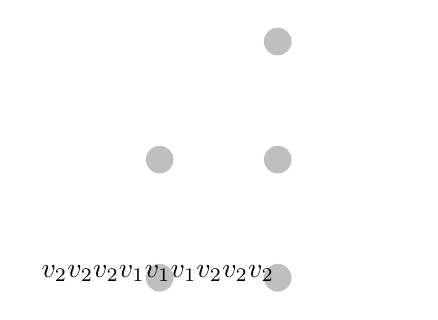
\begin{tikzpicture}[scale=\tikzpicscale]
    \node[Nvertex] (00) at (0,0)   {};
    \node[vertex] (10) at (1,0)   {};
	 \node[vertex] (20) at (2,0)   {};
%    \node[vertex] (01) at (0,1)   {};
    \node[vertex] (11) at (1,1)   {};
    \node[vertex] (21) at (2,1)   {};
%    \node[vertex] (02) at (0,2)   {};
%    \node[vertex] (12) at (1,2)   {};
    \node[vertex] (22) at (2,2)   {};
%	 \Edge[label=$v_2$](01)(10)
	 \Edge[label=$v_2$](10)(20)
%	 \Edge[label=$v_2$](01)(11)
	 \Edge[label=$v_2$](11)(21)
%	 \Edge[label=$v_2$](02)(12)
	 \Edge[label=$v_2$](11)(22)	
%)	 \Edge[label=$v_1$](00)(01)
	 \Edge[label=$v_1$](10)(11)
	 \Edge[label=$v_1$](20)(21)
 	 \Edge[label=$v_1$](21)(22)
% 	 \Edge[label=$v_1$](11)(02)
    \node[Nvertex] (n30) at (3,0)   {};
    \node[Nvertex] (n31) at (3,1)   {};
    \node[Nvertex] (n32) at (3,2)   {};
	 \tikzstyle{EdgeStyle}=[dashed]
	 \Edge[label=$v_2$](20)(n30)
	 \Edge[label=$v_2$](21)(n31)
 	 \Edge[label=$v_2$](22)(n32)
  	 %\tikzstyle{EdgeStyle}=[loop above]
  	 %\Edge[label=$v_1$](11)(11)
\end{tikzpicture}
}

\newcommand{\TIKZthreeladderG}{
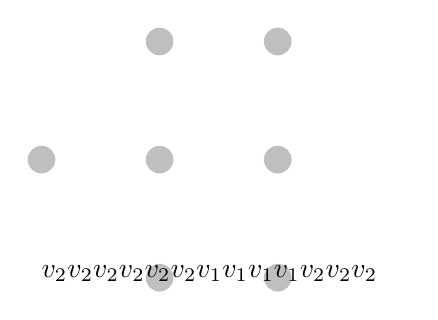
\begin{tikzpicture}[scale=\tikzpicscale]
%    \node[vertex] (00) at (0,0)   {};
    \node[vertex] (10) at (1,0)   {};
	 \node[vertex] (20) at (2,0)   {};
    \node[vertex] (01) at (0,1)   {};
    \node[vertex] (11) at (1,1)   {};
    \node[vertex] (21) at (2,1)   {};
%    \node[vertex] (02) at (0,2)   {};
    \node[vertex] (12) at (1,2)   {};
    \node[vertex] (22) at (2,2)   {};
	 \Edge[label=$v_2$](01)(10)
	 \Edge[label=$v_2$](10)(20)
	 \Edge[label=$v_2$](01)(11)
	 \Edge[label=$v_2$](11)(21)
	 \Edge[label=$v_2$](01)(12)
	 \Edge[label=$v_2$](12)(22)	
%)	 \Edge[label=$v_1$](00)(01)
	 \Edge[label=$v_1$](10)(11)
	 \Edge[label=$v_1$](20)(21)
 	 \Edge[label=$v_1$](21)(22)
 	 \Edge[label=$v_1$](11)(12)
% 	 \Edge[label=$v_1$](01)(02)
    \node[Nvertex] (n30) at (3,0)   {};
    \node[Nvertex] (n31) at (3,1)   {};
    \node[Nvertex] (n32) at (3,2)   {};
	 \tikzstyle{EdgeStyle}=[dashed]
	 \Edge[label=$v_2$](20)(n30)
	 \Edge[label=$v_2$](21)(n31)
 	 \Edge[label=$v_2$](22)(n32)
\end{tikzpicture}
}

\newcommand{\TIKZthreeladderH}{
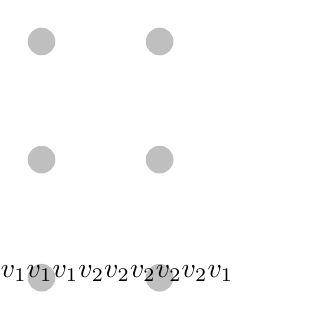
\begin{tikzpicture}[scale=\tikzpicscale]
%    \node[vertex] (00) at (0,0)   {};
    \node[vertex] (10) at (1,0)   {};
	 \node[vertex] (20) at (2,0)   {};
%    \node[vertex] (01) at (0,1)   {};
    \node[vertex] (11) at (1,1)   {};
    \node[vertex] (21) at (2,1)   {};
%    \node[vertex] (02) at (0,2)   {};
    \node[vertex] (12) at (1,2)   {};
    \node[vertex] (22) at (2,2)   {};
	 \Edge[label=$v_2$](10)(20)
%	 \Edge[label=$v_2$](01)(11)
	 \Edge[label=$v_2$](11)(21)
%	 \Edge[label=$v_2$](01)(12)
	 \Edge[label=$v_2$](12)(22)	
%)	 \Edge[label=$v_1$](00)(01)
	 \Edge[label=$v_1$](20)(21)
 	 \Edge[label=$v_1$](21)(22)
 	 \Edge[label=$v_1$](11)(12)
% 	 \Edge[label=$v_1$](01)(02)
    \node[Nvertex] (n30) at (3,0)   {};
    \node[Nvertex] (n31) at (3,1)   {};
    \node[Nvertex] (n32) at (3,2)   {};
	 \tikzstyle{EdgeStyle}=[dashed]
	 \Edge[label=$v_2$](20)(n30)
	 \Edge[label=$v_2$](21)(n31)
 	 \Edge[label=$v_2$](22)(n32)
 	 
 	 \tikzstyle{EdgeStyle}=[bend left]
 	 \Edge[label=$v_2$](10)(11)
  	 \tikzstyle{EdgeStyle}=[bend left=50]
 	 \Edge[label=$v_2$](10)(12)
  	 %\Edge[label=$v_2$](11)(12)
 	 \tikzstyle{EdgeStyle}=[bend right]
	 \Edge[label=$v_1$](10)(11)
\end{tikzpicture}
}

\newcommand{\TIKZthreeladderI}{
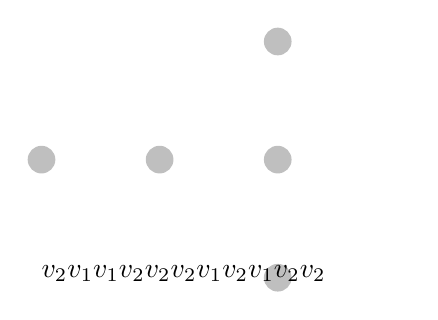
\begin{tikzpicture}[scale=\tikzpicscale]
%    \node[vertex] (00) at (0,0)   {};
%    \node[vertex] (10) at (1,0)   {};
	 \node[vertex] (20) at (2,0)   {};
    \node[vertex] (01) at (0,1)   {};
    \node[vertex] (11) at (1,1)   {};
    \node[vertex] (21) at (2,1)   {};
%    \node[vertex] (02) at (0,2)   {};
%    \node[vertex] (12) at (1,2)   {};
    \node[vertex] (22) at (2,2)   {};
%	 \Edge[label=$v_2$](01)(10)
%	 \Edge[label=$v_2$](10)(20)
%	 \Edge[label=$v_2$](01)(21)
	 \Edge[label=$v_2$](11)(21)
%	 \Edge[label=$v_2$](12)(22)	
%)	 \Edge[label=$v_1$](00)(01)
%	 \Edge[label=$v_1$](10)(11)
	 \Edge[label=$v_1$](20)(21)
 	 \Edge[label=$v_1$](21)(22)
% 	 \Edge[label=$v_1$](11)(12)
% 	 \Edge[label=$v_1$](01)(02)
    \node[Nvertex] (n30) at (3,0)   {};
    \node[Nvertex] (n31) at (3,1)   {};
    \node[Nvertex] (n32) at (3,2)   {};
	 \tikzstyle{EdgeStyle}=[dashed]
	 \Edge[label=$v_2$](20)(n30)
	 \Edge[label=$v_2$](21)(n31)
 	 \Edge[label=$v_2$](22)(n32)

	 \tikzstyle{EdgeStyle}=[]
	 \Edge[label=$v_1$](01)(11)
  	 \tikzstyle{EdgeStyle}=[bend left=50]
	 \Edge[label=$v_2$](01)(22)
 	 \Edge[label=$v_1$](01)(11)
  	 \tikzstyle{EdgeStyle}=[bend right=50]
 	 \Edge[label=$v_2$](01)(20)
 	 \Edge[label=$v_2$](01)(11)
\end{tikzpicture}
}


\newcommand{\TIKZthreeladderJ}{
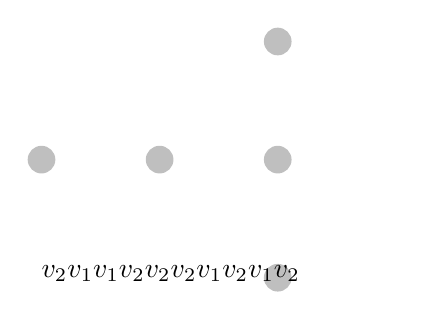
\begin{tikzpicture}[scale=\tikzpicscale]
%    \node[vertex] (00) at (0,0)   {};
%    \node[vertex] (10) at (1,0)   {};
	 \node[vertex] (20) at (2,0)   {};
    \node[vertex] (01) at (0,1)   {};
    \node[vertex] (11) at (1,1)   {};
    \node[vertex] (21) at (2,1)   {};
%    \node[vertex] (02) at (0,2)   {};
%    \node[vertex] (12) at (1,2)   {};
    \node[vertex] (22) at (2,2)   {};
%	 \Edge[label=$v_2$](01)(10)
%	 \Edge[label=$v_2$](10)(20)
%	 \Edge[label=$v_2$](01)(21)
	 \Edge[label=$v_2$](11)(21)
%	 \Edge[label=$v_2$](12)(22)	
%)	 \Edge[label=$v_1$](00)(01)
%	 \Edge[label=$v_1$](10)(11)
	 \Edge[label=$v_1$](20)(21)
 	 \Edge[label=$v_1$](21)(22)
% 	 \Edge[label=$v_1$](11)(12)
% 	 \Edge[label=$v_1$](01)(02)
    \node[Nvertex] (n30) at (3,0)   {};
    \node[Nvertex] (n31) at (3,1)   {};
    \node[Nvertex] (n32) at (3,2)   {};
	 \tikzstyle{EdgeStyle}=[dashed]
	 \Edge[label=$v_2$](20)(n30)
	 \Edge[label=$v_2$](21)(n31)
 	 \Edge[label=$v_2$](22)(n32)

	 \tikzstyle{EdgeStyle}=[]
	 \Edge[label=$v_1$](01)(11)
  	 \tikzstyle{EdgeStyle}=[bend left=50]
	 \Edge[label=$v_2$](01)(22)
 	 \Edge[label=$v_1$](01)(11)
  	 \tikzstyle{EdgeStyle}=[bend right=50]
 	 \Edge[label=$v_2$](01)(20)
% 	 \Edge[label=$v_2$](01)(11)
\end{tikzpicture}
}

\newcommand{\TIKZoneladderA}{
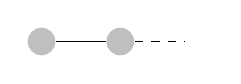
\begin{tikzpicture}[shorten >=1pt,->]
    \tikzstyle{vertex}=[circle,fill=black!25,minimum size=10pt,inner sep=2pt]
    \tikzstyle{nullvertex}=[circle,fill=white!25,minimum size=10pt,inner sep=2pt]
    \node[vertex] (G1) at (0,0)   {};
    \node[vertex] (G2) at (1,0)   {};
    \node[nullvertex] (GX) at (2,0)   {};
    \draw (G1) -- (G2) -- cycle;
    \draw[dashed] (G2) -- (GX) -- cycle;
\end{tikzpicture}
}

\newcommand{\TIKZoneladderB}{
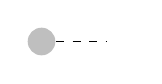
\begin{tikzpicture}[shorten >=1pt,->]
    \tikzstyle{vertex}=[circle,fill=black!25,minimum size=10pt,inner sep=2pt]
    \tikzstyle{nullvertex}=[circle,fill=white!25,minimum size=10pt,inner sep=2pt]
    \node[vertex] (G2) at (1,0)   {};
    \node[nullvertex] (GX) at (2,0)   {};
    \draw[dashed] (G2) -- (GX) -- cycle;
\end{tikzpicture}
}

\newcommand{\TIKZoneladderC}{

\begin{tikzpicture}[shorten >=1pt,->]
    \tikzstyle{vertex}=[circle,fill=black!25,minimum size=10pt,inner sep=2pt]
    \tikzstyle{nullvertex}=[circle,fill=white!25,minimum size=10pt,inner sep=2pt]
    \node[vertex] (G1) at (0,0)   {};
    \node[vertex] (G2) at (1,0)   {};
    \node[nullvertex] (GX) at (2,0)   {};
    %\draw (G1) -- (G2) -- cycle;
    \draw[dashed] (G2) -- (GX) -- cycle;
\end{tikzpicture}
}

\newcommand{\TIKZpetersengraph} {
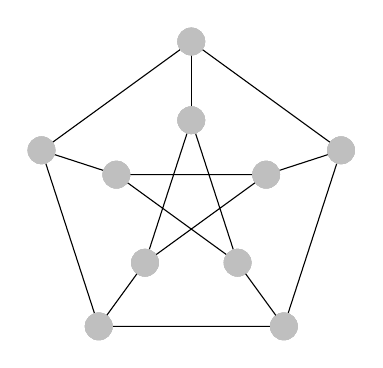
\begin{tikzpicture}[]
    \tikzstyle{vertex}=[circle,fill=black!25,minimum size=10pt,inner sep=2pt]
            
\draw (18:2cm) -- (90:2cm) -- (162:2cm) -- (234:2cm) -- (306:2cm) -- cycle;
\draw (18:1cm) -- (162:1cm) -- (306:1cm) -- (90:1cm) -- (234:1cm) -- cycle;
\foreach \x in {18,90,162,234,306}{
\draw (\x:1cm) -- (\x:2cm);

    \node[vertex] at (18:2cm) {};
    \node[vertex] at (90:2cm) {};
    \node[vertex] at (162:2cm) {};
    \node[vertex] at (234:2cm) {};
    \node[vertex] at (306:2cm) {};
    \node[vertex] at (18:1cm) {};
    \node[vertex] at (162:1cm) {};
    \node[vertex] at (306:1cm) {};
    \node[vertex] at (90:1cm) {};
    \node[vertex] at (234:1cm) {};

%\draw (\x:2cm) circle (2pt);
%\draw (\x:1cm) circle (2pt);
}
\end{tikzpicture}
}

\newcommand{\TIKZFLWmacrostates} {

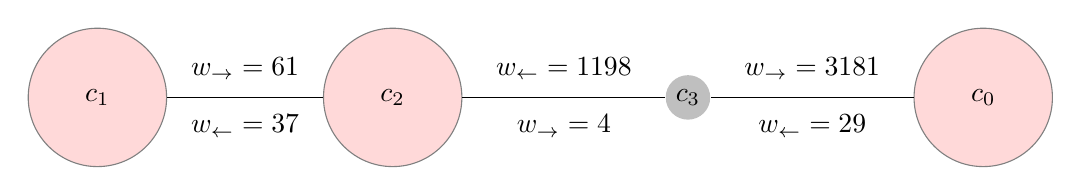
\begin{tikzpicture}[scale=\tikzpicscale]

  \node[big_vertex] (c1) at (0,0)   {$c_1$};
  \node[big_vertex] (c2) at (1*\vertexshiftamount,0)   {$c_2$};
  \node[vertex]    (c3) at (2*\vertexshiftamount,0)   {$c_3$};
  \node[big_vertex] (c0) at (3*\vertexshiftamount,0)   {$c_0$};
  
  \draw [] (c0) -> node[above=.1cm] {$w_{\rightarrow}=3181$} (c3);
  \draw [] (c0) -> node[below=.1cm] {$w_{\leftarrow}=29$} (c3);

  \draw [] (c2) -> node[above=.1cm] {$w_{\leftarrow}=1198$} (c3);  
  \draw [] (c2) -> node[below=.1cm] {$w_{\rightarrow}=4$} (c3);
  
  \draw [] (c2) -- node[below=.1cm] {$w_{\leftarrow}=37$} (c1);
  \draw [] (c2) -- node[above=.1cm] {$w_{\rightarrow}=61$} (c1);
\end{tikzpicture}
}

\newcommand{\TIKZbetahairpinNativestate} {
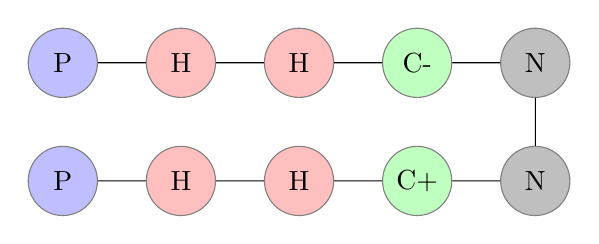
\begin{tikzpicture}[scale=\tikzpicscale]
    \tikzstyle{hvertex}=[circle,fill=red!25,minimum size=25pt,inner sep=2pt,draw=black!50]
    \tikzstyle{pvertex}=[circle,fill=blue!25,minimum size=25pt,inner sep=2pt,draw=black!50]
    \tikzstyle{cpvertex}=[circle,fill=green!25,minimum size=25pt,inner sep=2pt,draw=black!50]
    \tikzstyle{nvertex}=[circle,fill=black!25,minimum size=25pt,inner sep=2pt,draw=black!50]

    \node[pvertex] (r0) at (0,0)   {\chem{P}};
    \node[hvertex] (r1) at (1,0)   {\chem{H}};
    \node[hvertex] (r2) at (2,0)   {\chem{H}};
    \node[cpvertex] (r3) at (3,0)   {\chem{C+}};
    \node[nvertex] (r4) at (4,0)   {\chem{N}};
    \node[nvertex] (r5) at (4,1)   {\chem{N}};
    \node[cpvertex] (r6) at (3,1)   {\chem{C-}};
    \node[hvertex] (r7) at (2,1)   {\chem{H}};
    \node[hvertex] (r8) at (1,1)   {\chem{H}};
    \node[pvertex] (r9) at (0,1)   {\chem{P}};

    \draw [] (r0)--(r1)--(r2)--(r3)--(r4)--(r5)--(r6)--(r7)--(r8)--(r9)--cycle;
   
\end{tikzpicture}
}


\newcommand{\TIKZbetahairpinMacrostates} {
\begin{tikzpicture}[scale=\tikzpicscale]
    \node[macrostate_vertex] (R) at (0,0)   {
    \begin{minipage}{3.1cm}
    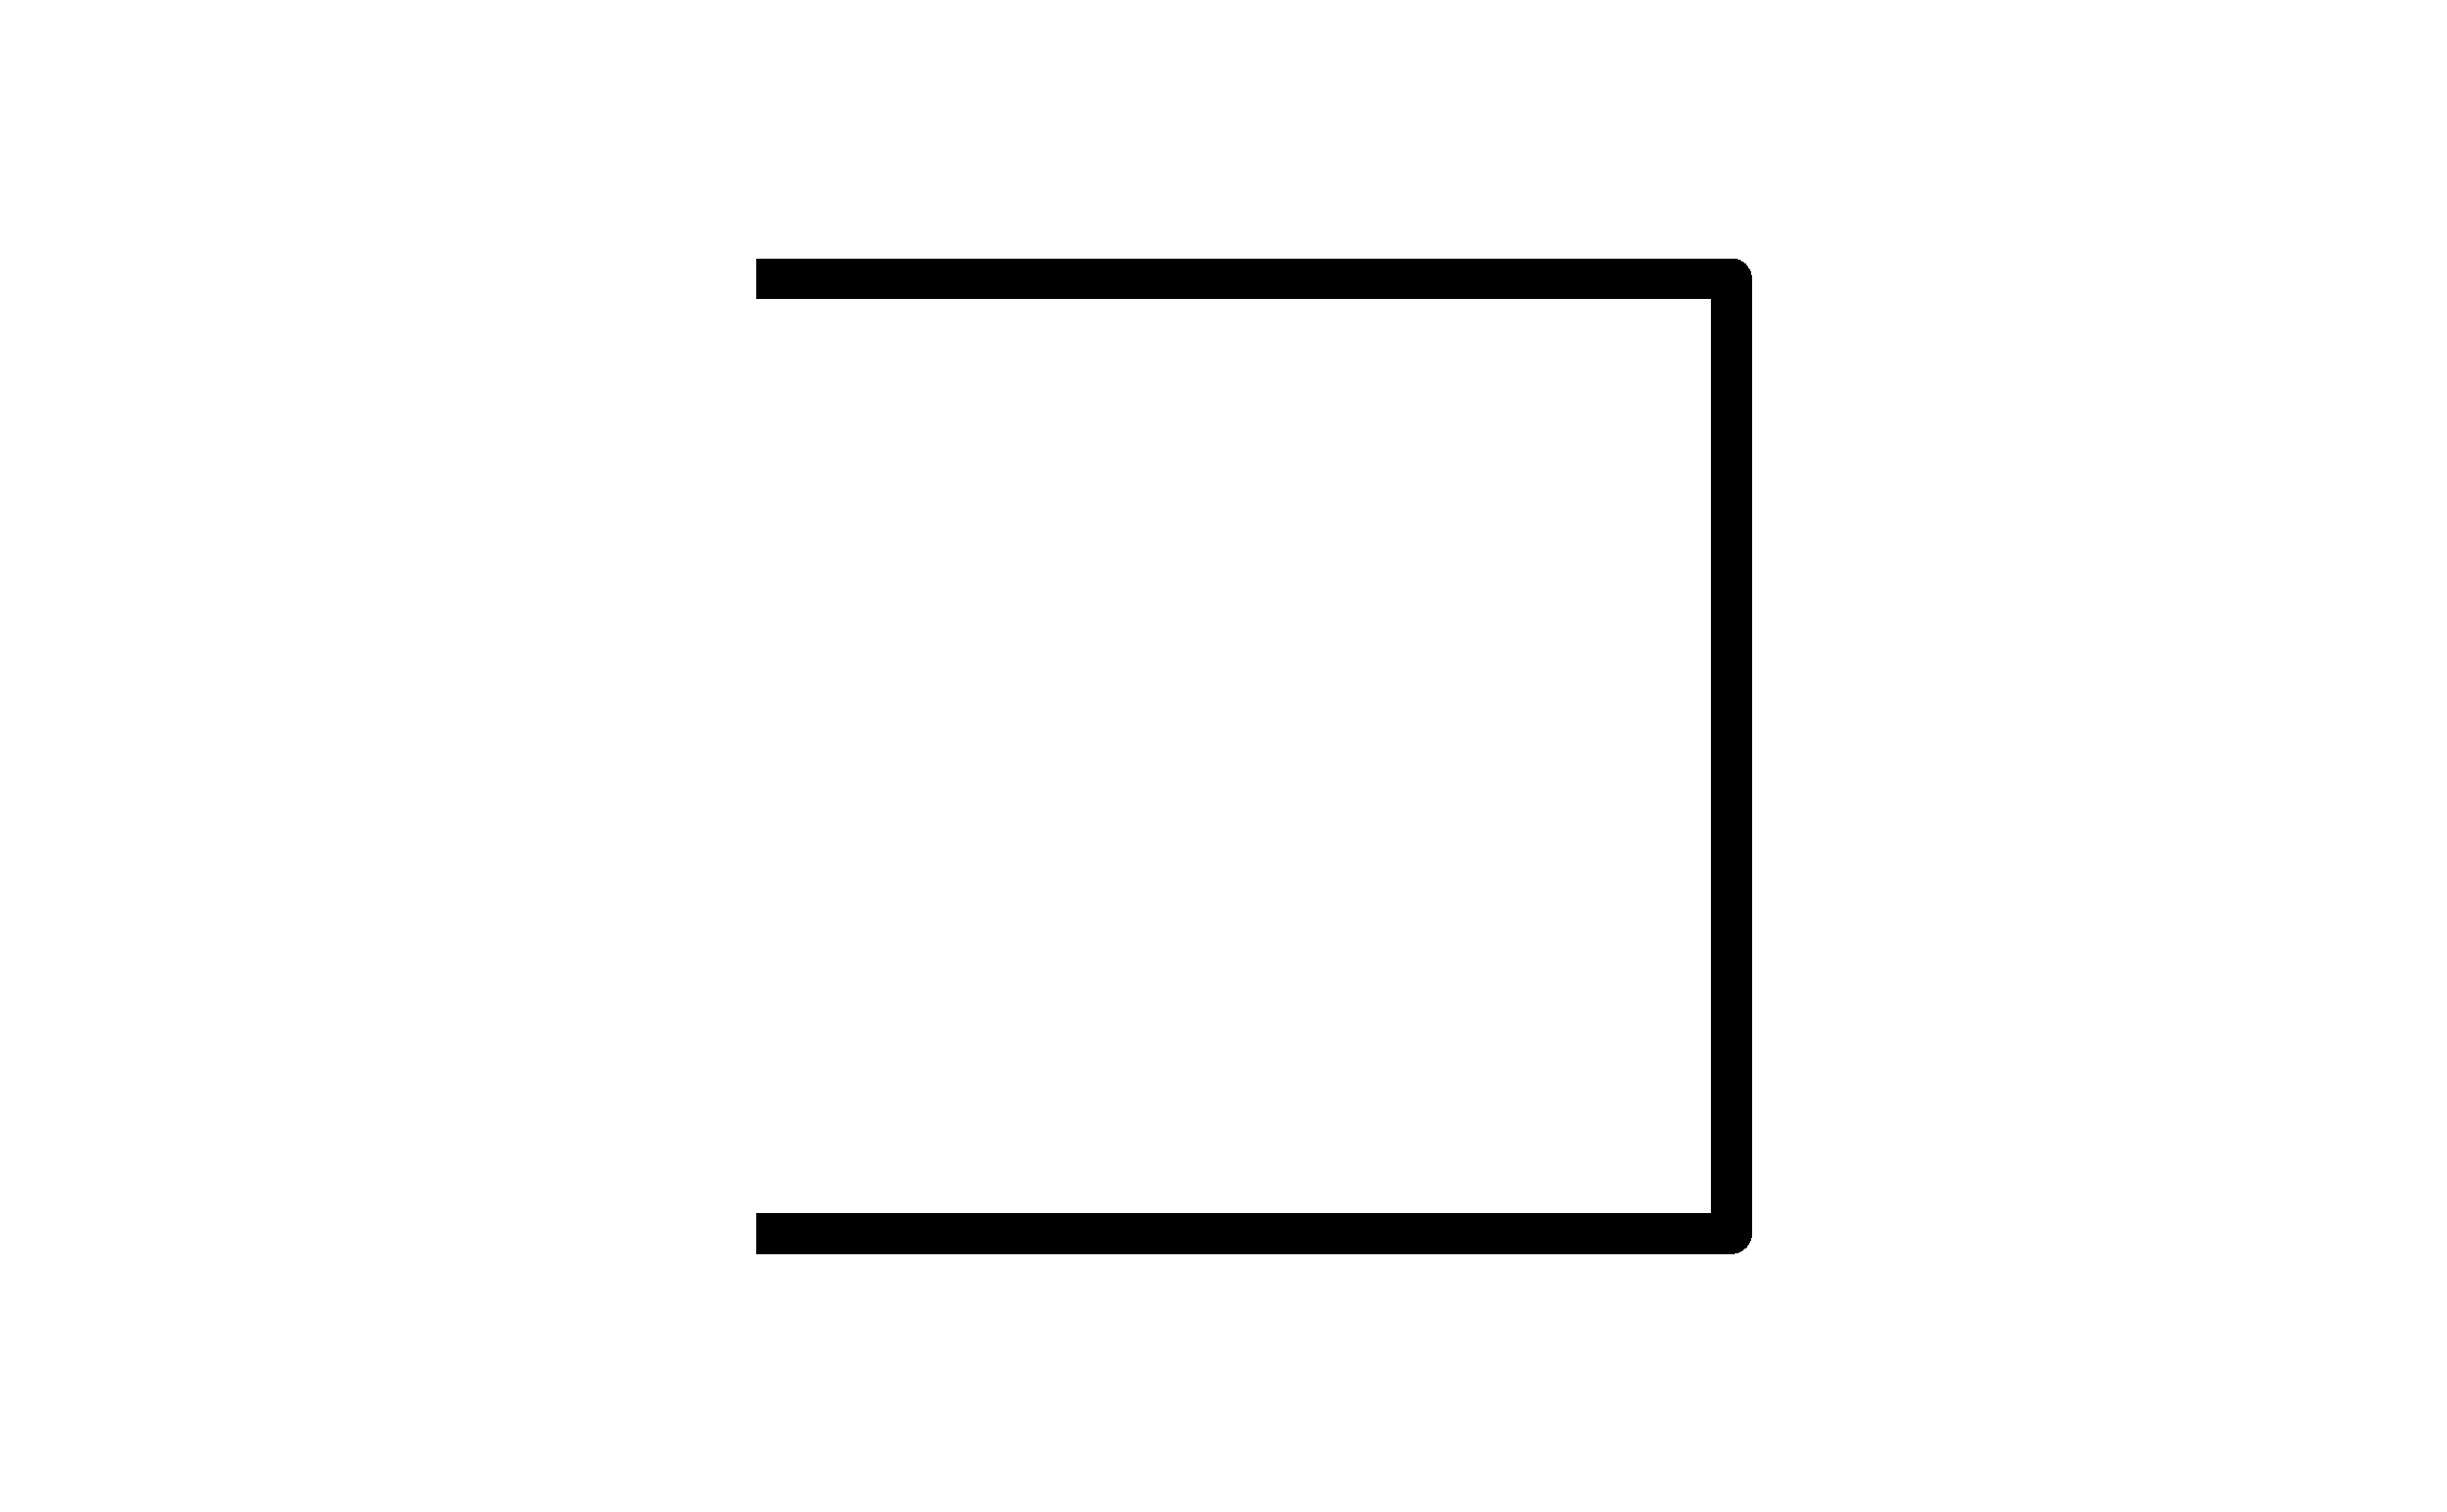
\includegraphics[width=1.5 cm]{supplement/beta_cluster_example_2/pictures/21/state_cluster_shapes_150.pdf} 
    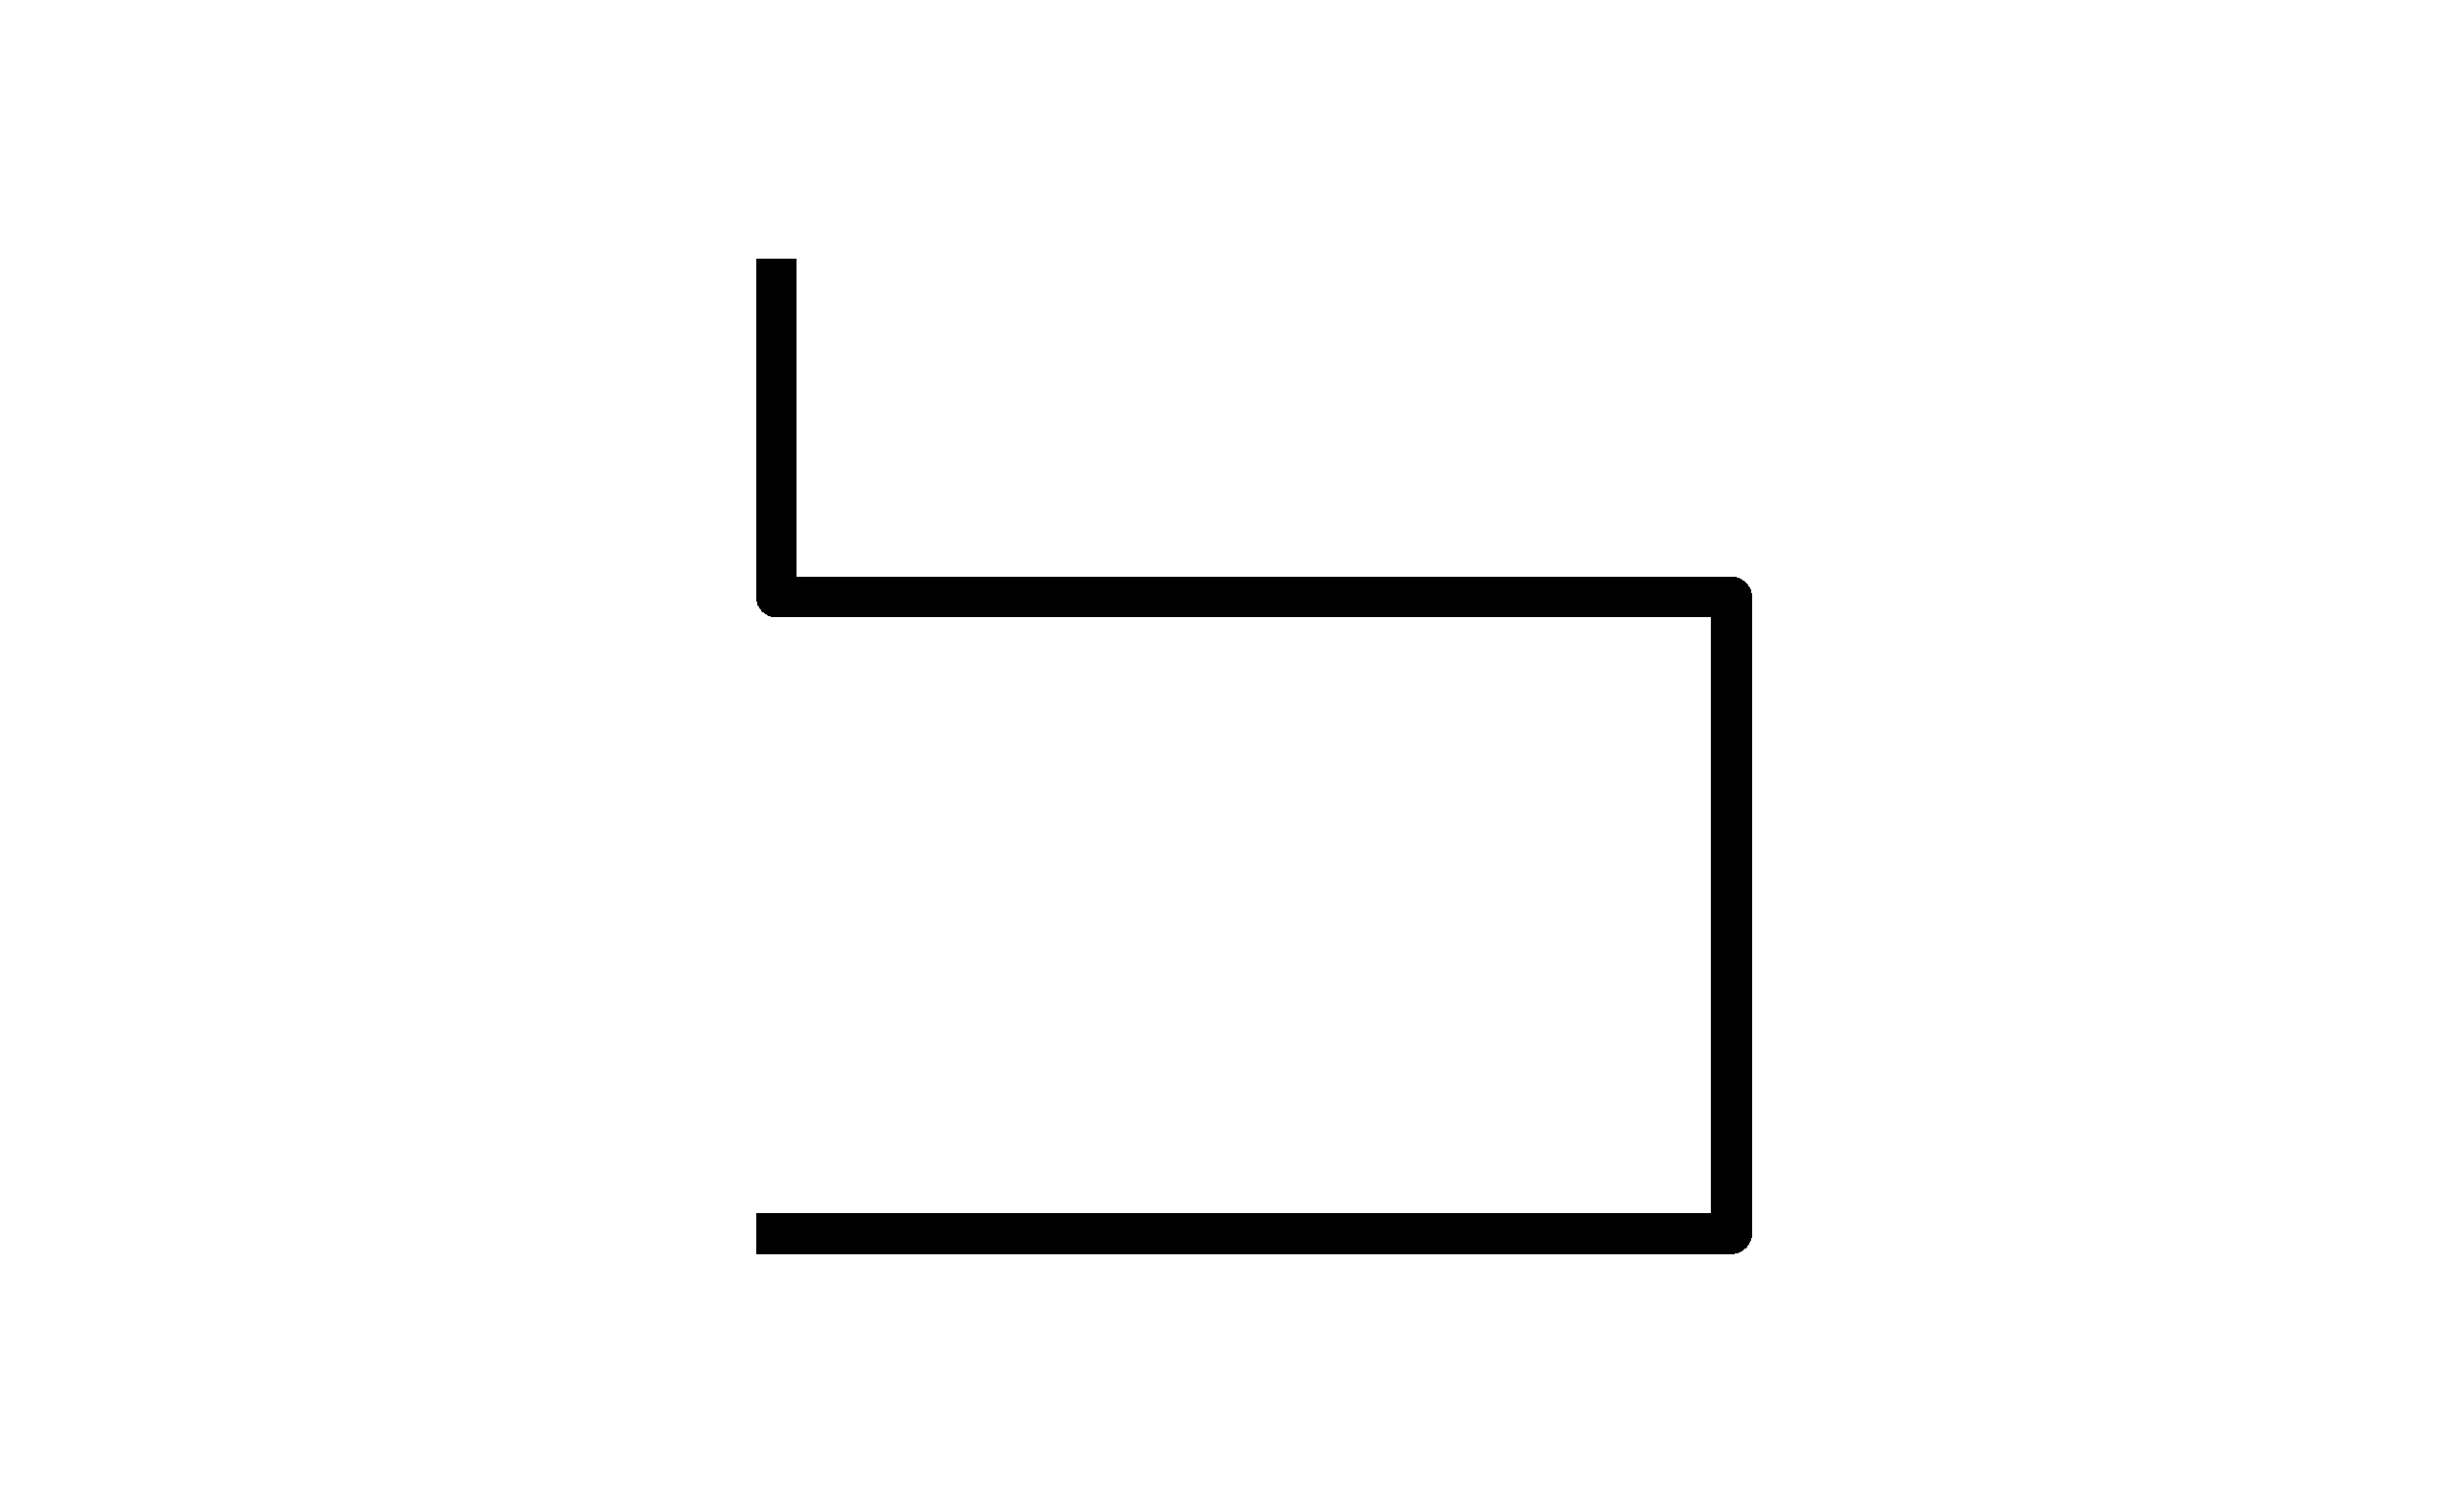
\includegraphics[width=1.5 cm]{supplement/beta_cluster_example_2/pictures/21/state_cluster_shapes_17.pdf} \\
    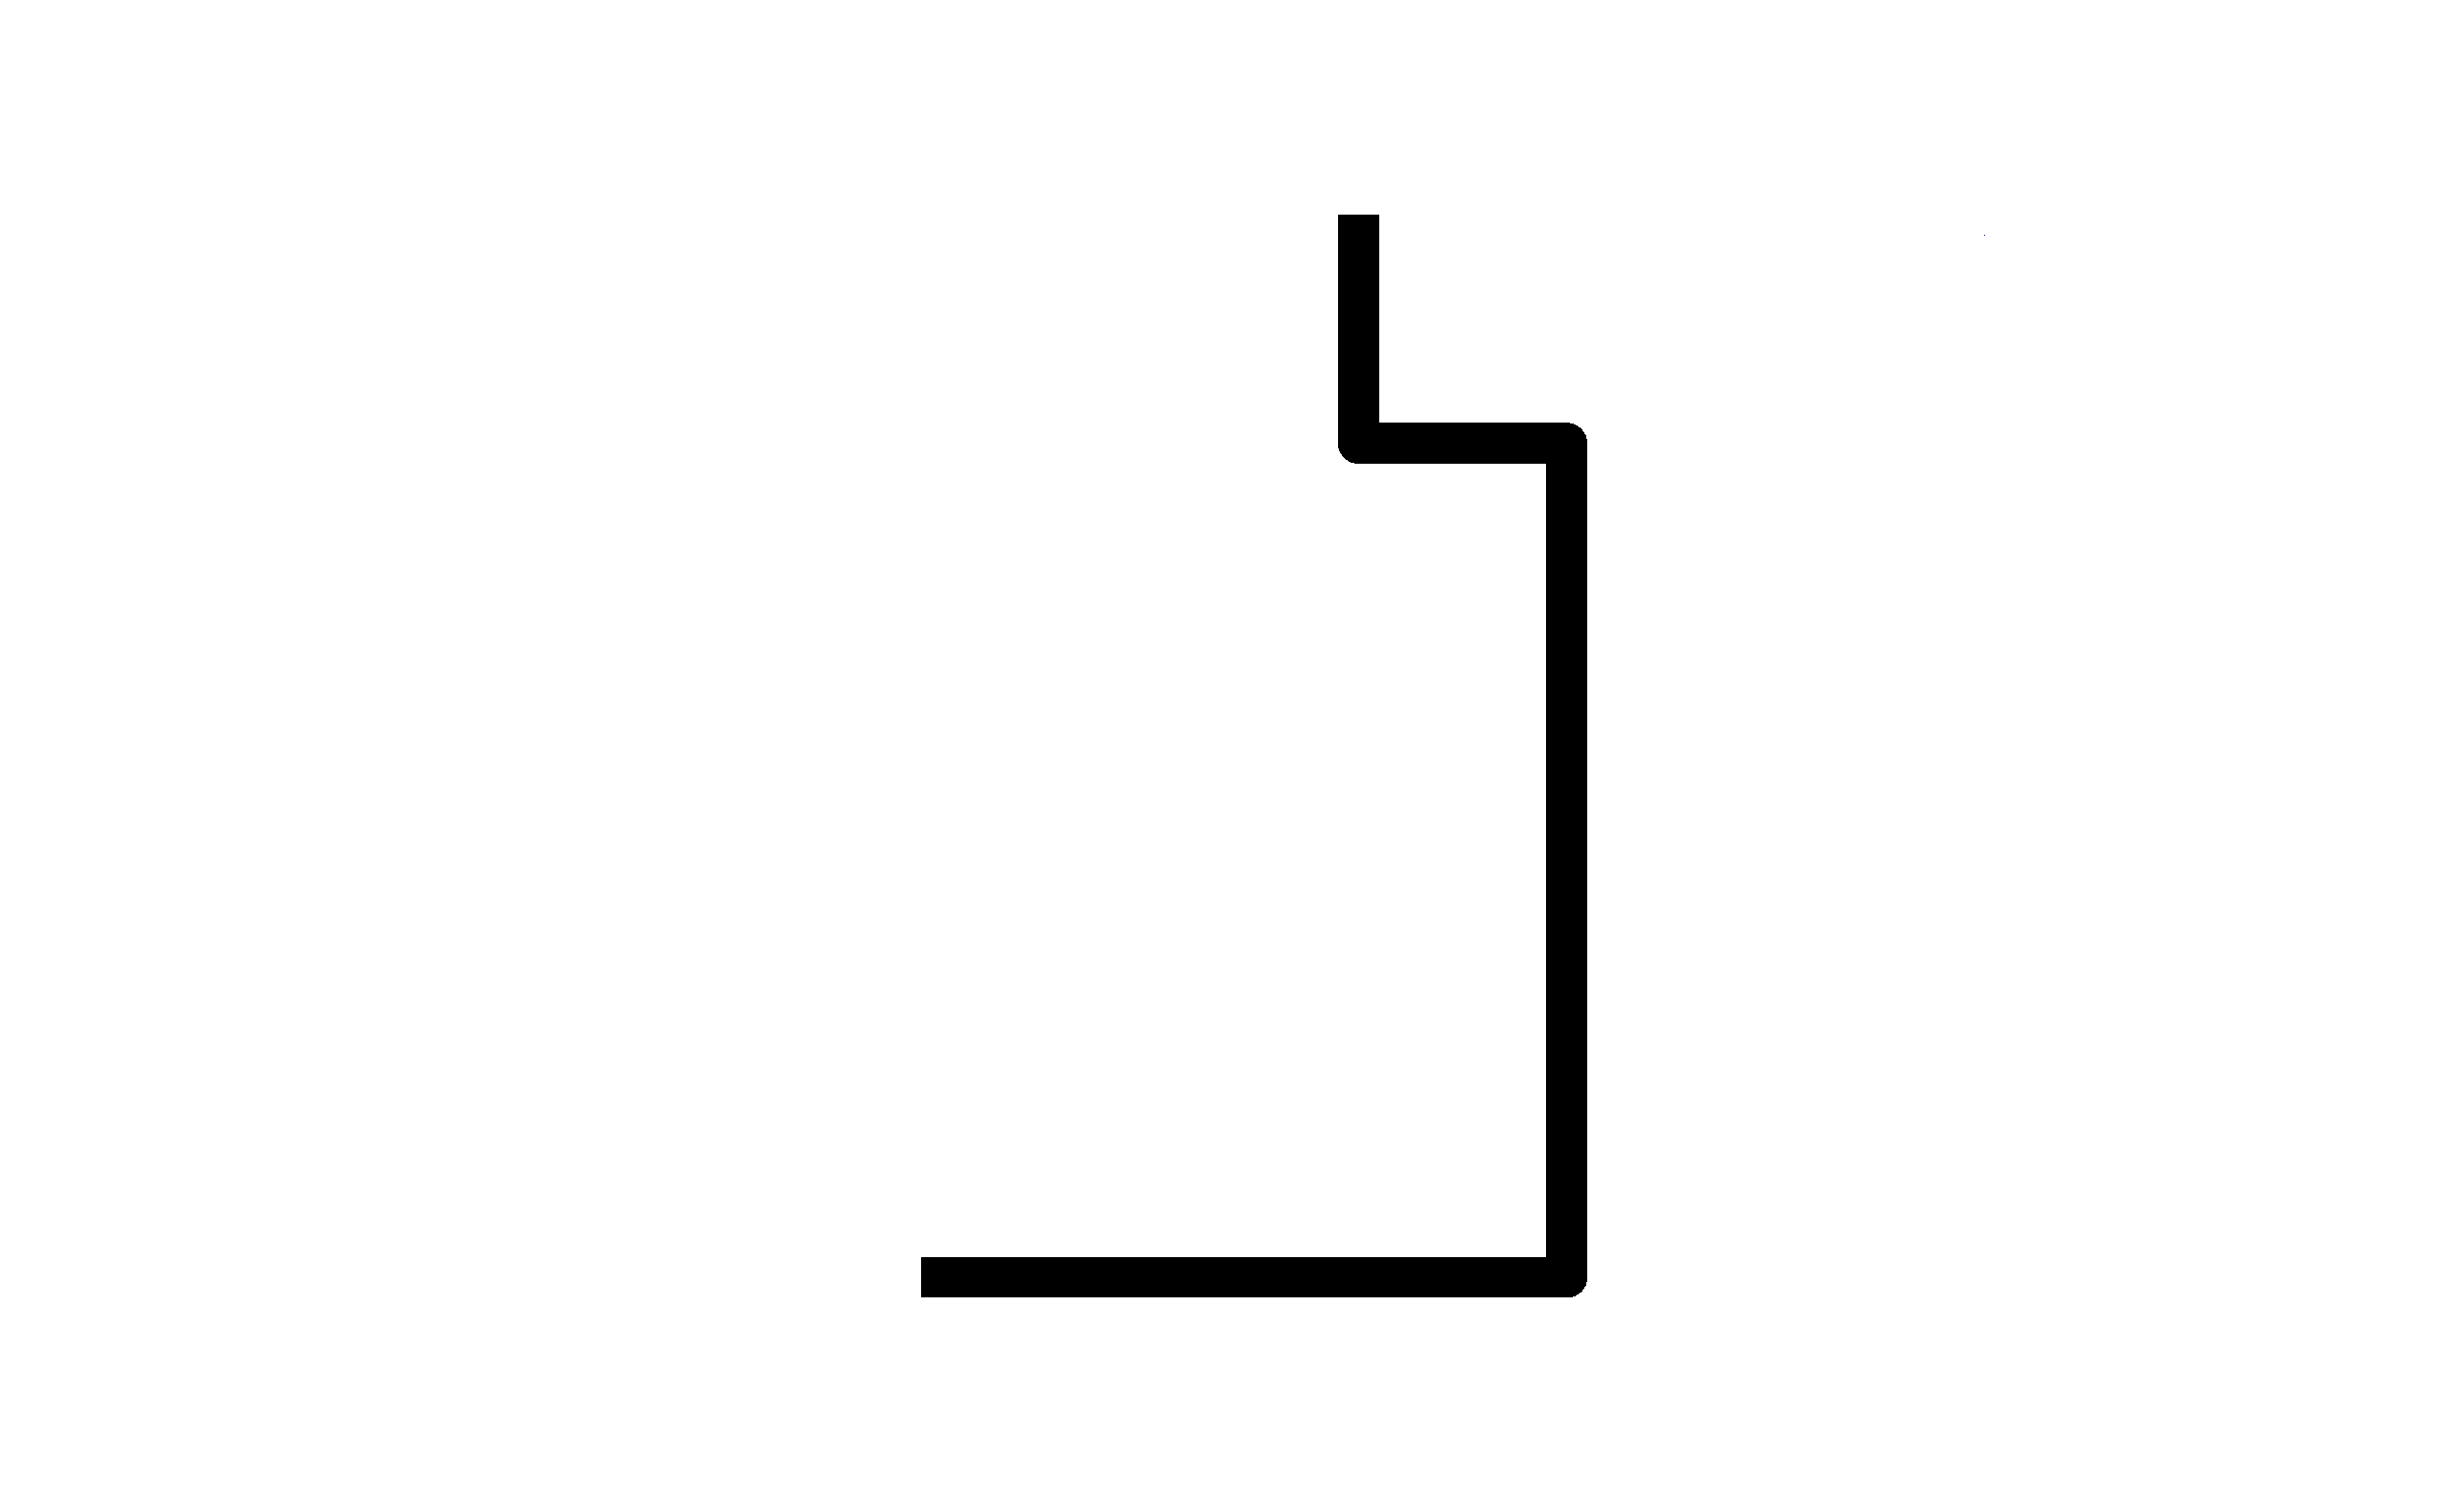
\includegraphics[width=1.5 cm]{supplement/beta_cluster_example_2/pictures/21/state_cluster_shapes_32.pdf} 
    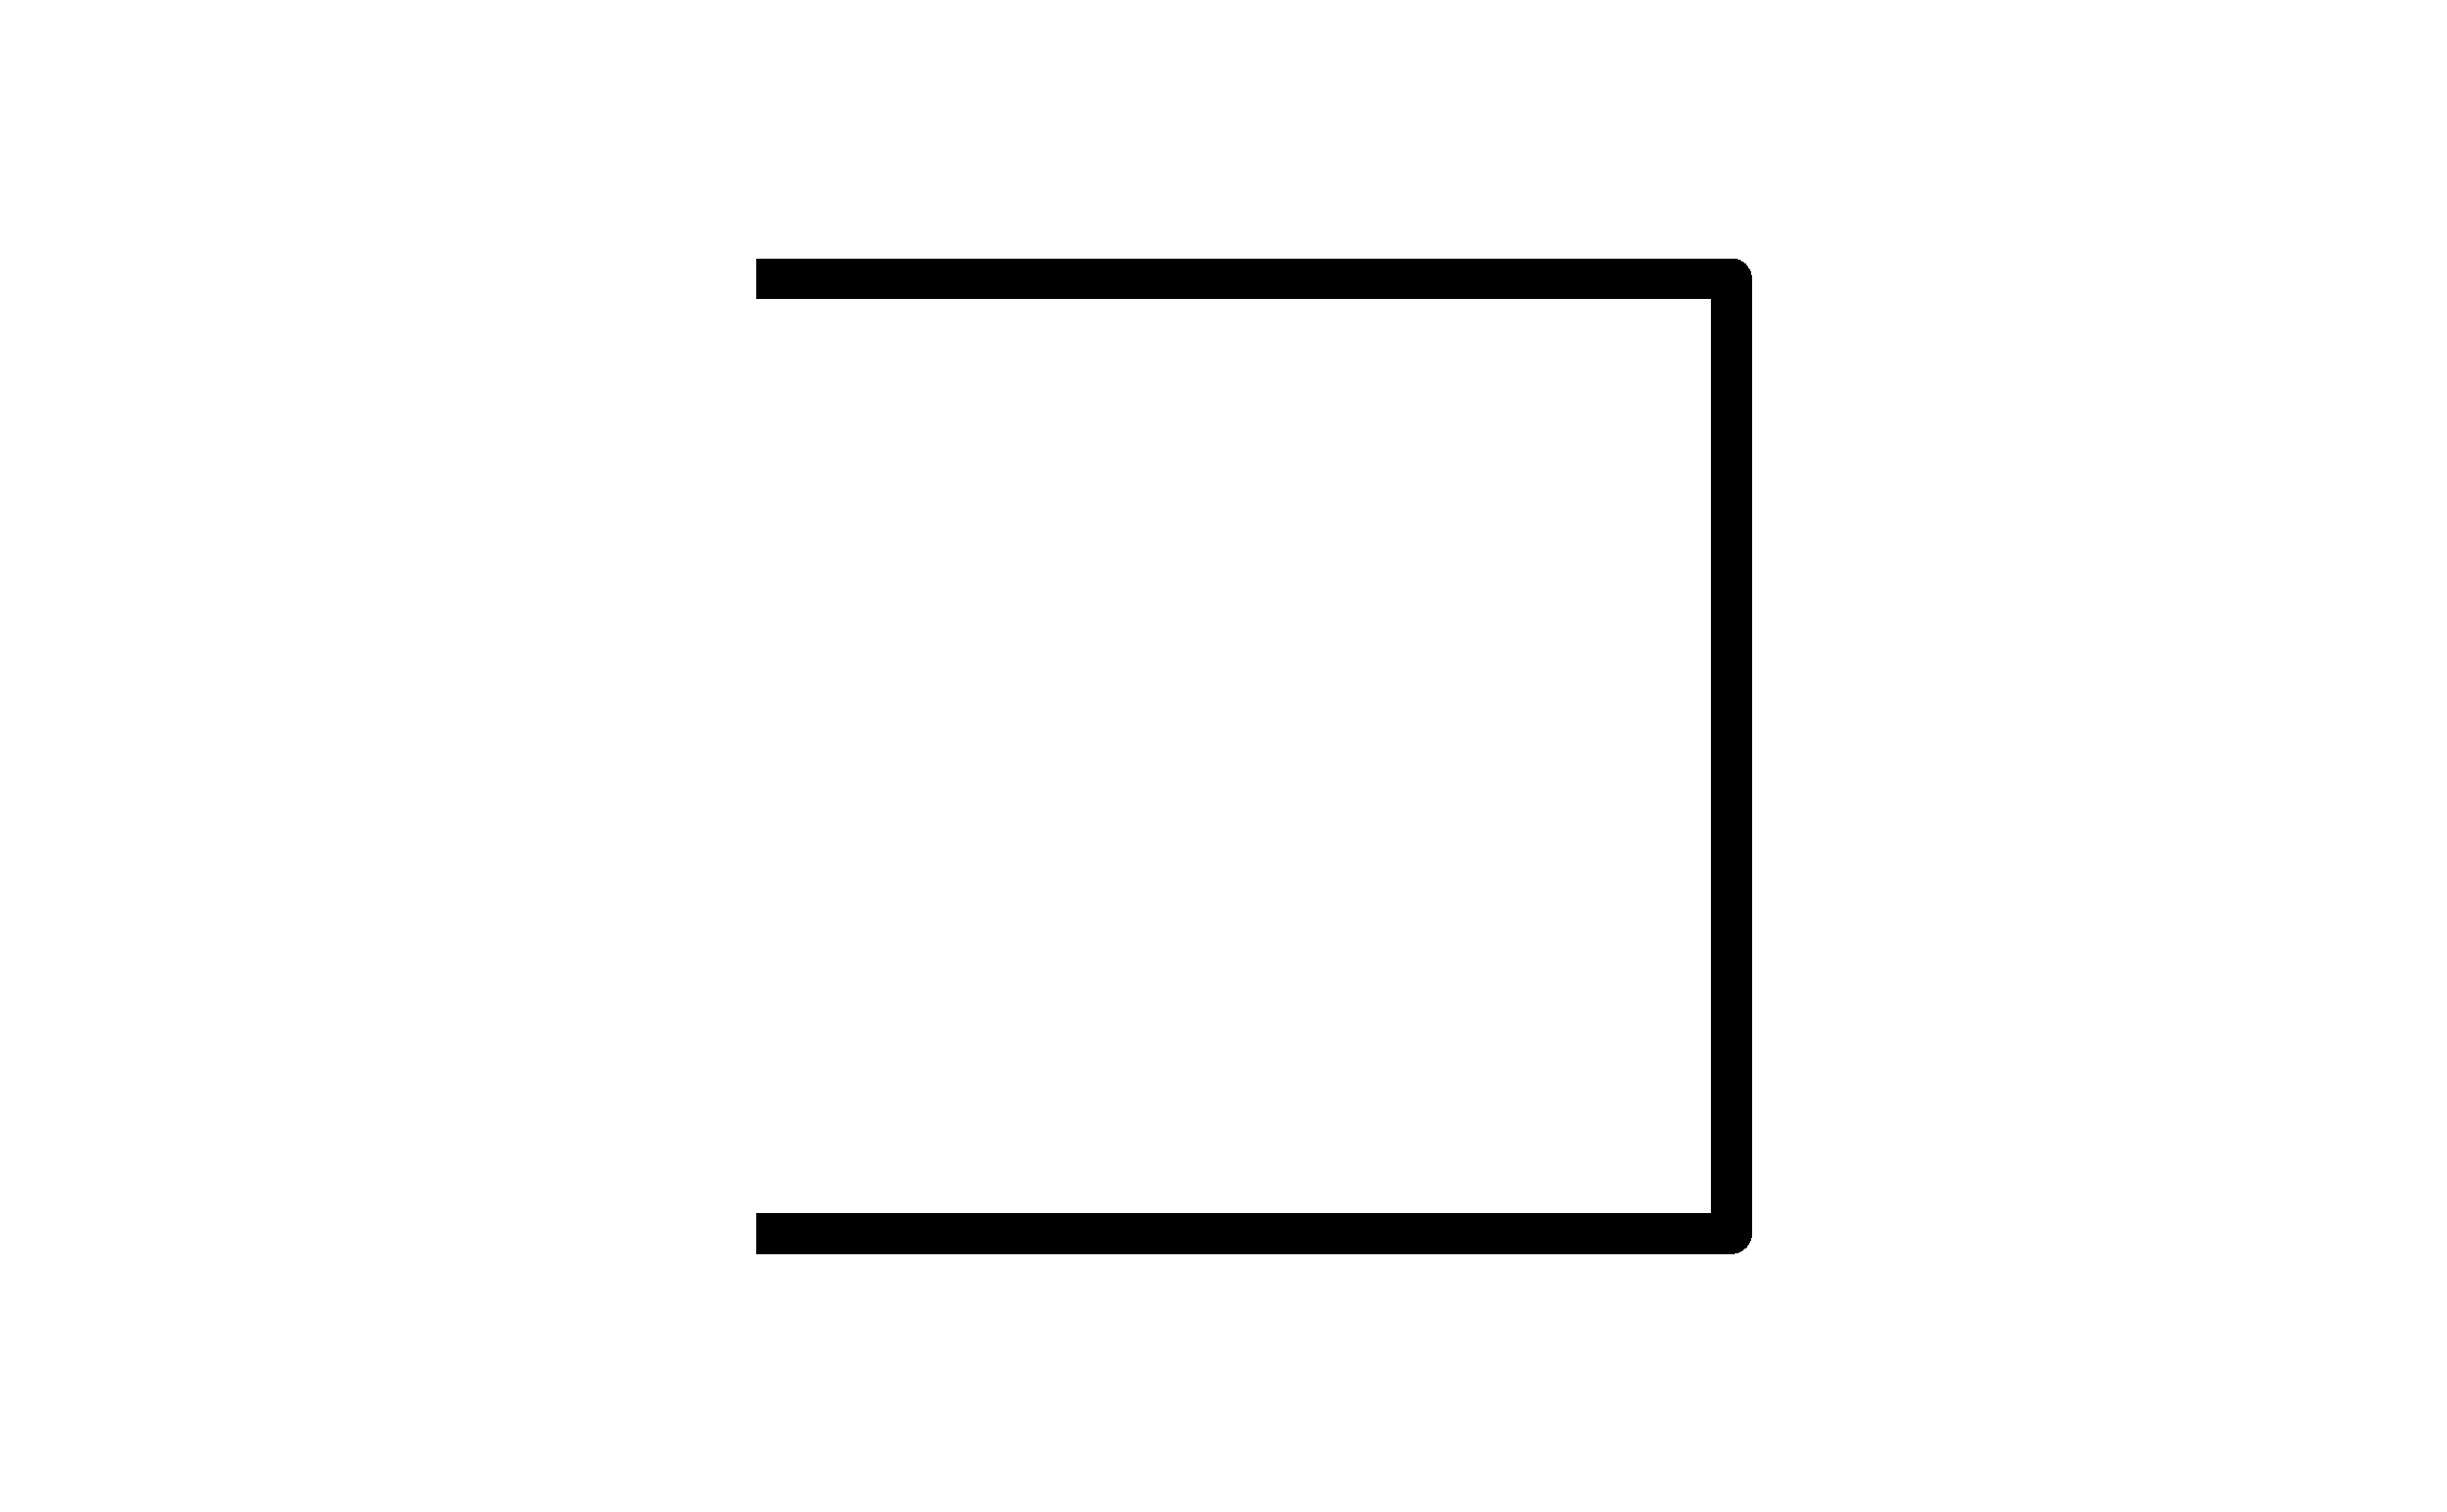
\includegraphics[width=1.5 cm]{supplement/beta_cluster_example_2/pictures/21/state_cluster_shapes_200.pdf} \\
  	 $c_\chem{R}$ random coil
    \end{minipage}
    };
    \node[macrostate_vertex] (I) at (1.5*\vertexshiftamount,0)   {
    \begin{minipage}{3.1cm} \centering
    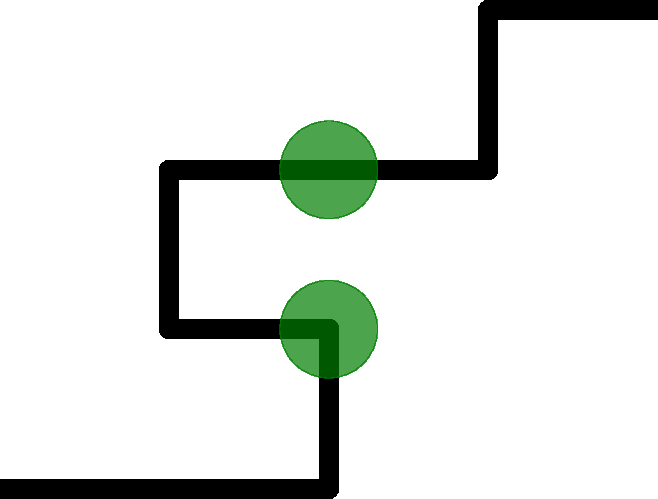
\includegraphics[width=2 cm]{supplement/beta_cluster_example_2/pictures/saved_macrostates/intermed.png} \\
  	 $c_\chem{I}$ intermediate \\ (turn formation)
    \end{minipage}
	 };
    \node[macrostate_vertex] (F) at (3*\vertexshiftamount,0)   
    {
    \begin{minipage}{3.1cm} \centering
    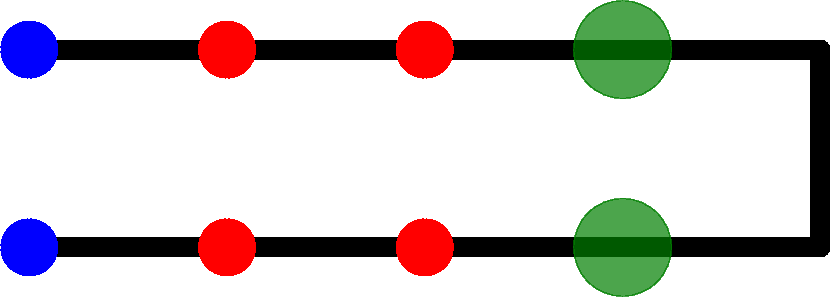
\includegraphics[width=2.5 cm]{supplement/beta_cluster_example_2/pictures/saved_macrostates/native.png} \\
  	 $c_\chem{F}$ native state
    \end{minipage}
    };

  \tikzstyle{EdgeStyle}=[bend right]
  \Edge[label=$\B{S}_{\chem{R I}}$](R)(I)
  \Edge[label=$\B{S}_{\chem{I R}}$](I)(R)
  
  \tikzstyle{EdgeStyle}=[]
  \Edge[label=$\B{S}_{\chem{I F}}$](I)(F)
  
\end{tikzpicture}
}


%\end{comment}
